\documentclass[12pt]{article}
% controlling the geometry of the page:
\usepackage[margin=1in, paperwidth=8.5in, paperheight=11in]{geometry} 
\usepackage{amsmath, amssymb} % useful math symbols and environments

\usepackage{multicol} % multiple columns side-by-side

\usepackage{amsthm} % Theorem-like environments
\theoremstyle{definition} % Without this line, theorem statements (and therefore problem statements etc.) show up in italic text.
\newtheorem{conjecture}{Conjecture}
\newtheorem{problem}{Problem}

% pretty colors!
\usepackage[dvipsnames]{xcolor}
\colorlet{darkgrey}{black!70}
\colorlet{darkgreen}{green!50!black}

\usepackage{tikz} % for drawing diagrams
\usetikzlibrary{arrows,automata,positioning} 
\usetikzlibrary{decorations.markings}
\usetikzlibrary{decorations.pathreplacing}
\usetikzlibrary{patterns}
\usetikzlibrary{shapes.geometric}

%%---------------------------------------------------------------------------
%% included from visualalgebra.sty (see the beamer folder)
%% TEXT COLORS
%%
\definecolor{xRed}{rgb}{.9,0,0}       
\definecolor{xBlue}{rgb}{0,0,.9}      
\definecolor{xGreen}{HTML}{009000}   %% "Islamic green"
\definecolor{xPurple}{HTML}{D14FFF}  
\definecolor{xOrange}{HTML}{F56600}  %% "Clemson orange"

\newcommand{\Alert}[1]{\textcolor{xRed}{#1}}
\newcommand{\Balert}[1]{\textcolor{xBlue}{#1}}
\newcommand{\Galert}[1]{\textcolor{xGreen}{#1}}
\newcommand{\Palert}[1]{\textcolor{xPurple}{#1}}
\newcommand{\Oalert}[1]{\textcolor{xOrange}{#1}}
\newcommand{\Walert}[1]{\textcolor{white}{#1}}

%% vertices in cayley graphs
\tikzset{v/.style={circle, draw, fill=lightgray,inner sep=0pt, 
  minimum size=6mm}}

%% Edge colors
%%
\definecolor{eRed}{rgb}{1,0,0}      % Cayley diagram edges
\definecolor{eBlue}{rgb}{0,0,1}     % Cayley diagram edges
\definecolor{eGreen}{HTML}{7EC636}  % Goodnotes green (a little darker)
\definecolor{eGreen}{HTML}{3CAC13}  % I like this a litte better
\definecolor{ePurple}{HTML}{D287FF} % Close to goodnotes 
\colorlet{eOrange}{orange}

%% Edge styles 
%%
\tikzset{r/.style={draw, very thick, eRed, -stealth}}  % Red -->
\tikzset{rr/.style={draw, very thick, eRed}}           % Red ---
\tikzset{b/.style={draw, very thick, eBlue, -stealth}} % Blue -->
\tikzset{bb/.style={draw, very thick, eBlue}}          % Blue ---
\tikzset{g/.style={draw, very thick, eGreen, -stealth}} % Green -->
\tikzset{gg/.style={draw, very thick, eGreen}}          % Green ---
%%---------------------------------------------------------------------------

\usepackage{graphicx} % for inserting figures with \includegraphics
\usepackage{setspace} % for controlling space between lines, paragraphs, etc.

\usepackage{fancyhdr} % for controlling headers and footers
\usepackage{newtx} % changes the default font family
\usepackage[shortlabels]{enumitem} % controllable labels for ordered and unordered lists

\usepackage{hyperref} % controls hyperlinks, both internal and external
\hypersetup{
    colorlinks=true,
    urlcolor=blue,
}

\setlength{\headheight}{14.5pt}
\newcommand{\Q}{\mathbb{Q}}
\newcommand{\R}{\mathbb{R}}
\newcommand{\Z}{\mathbb{Z}}
\newcommand\inv{^{-1}} % I am very tired of typing ^{-1}
\def\<{\langle}
\def\>{\rangle}
\DeclareMathOperator\Rect{\mathbf{Rect}}
\DeclareMathOperator\Tri{\mathbf{Tri}}
\DeclareMathOperator\Sq{\mathbf{Sq}}
\DeclareMathOperator\Light{\mathbf{Light}}
\DeclareMathOperator{\lcm}{lcm}

\newenvironment{red}{\color{red}}{\ignorespacesafterend}

% I don't like how LaTeX renders section headings by default
\renewcommand{\section}[1]{\begin{center} \textbf{#1} \\\end{center}}
%
\setlength{\parindent}{0in}
%\oddsidemargin=-.25in
\allowdisplaybreaks
\pagestyle{fancy}
\renewcommand{\headrulewidth}{0pt}
\lhead{MATH 312}
\rhead{Spring 2025}
%\lfoot{\copyright\ CLEAR Calculus 2010}
\cfoot{}
\renewcommand{\thefootnote}{*} 
\hyphenpenalty=10000 % LaTeX by default really likes hyphenating things

% all the stuff above this line is called the preamble...
%##################################################################
\begin{document} % this is always the first line of what's actually produced
\section{Homework \#4} % notice that if you want the character # to appear, you have to "escape" it with a backslash

HW due Sunday 2/16 by pdf upload to Canvas; .tex source on the \href{https://github.com/rhinopotamus/math312}{MATH 312 github repo}.


\subsection*{General facts about subgroups}

\begin{problem}[the one-step subgroup test]\label{onestep}
    A subset $H\subseteq G$ is a subgroup \Alert{if and only if} the following condition holds:
    \begin{equation}
        \text{If } x, y \in H, \text{ then } xy^{-1}\in H.
    \end{equation}
    Prove it! Hint: 
    \begin{multicols}{2}
        ($\Rightarrow$) Suppose that $H\leq G$.

        \ldots

        Therefore, whenever $x, y \in H$, $xy\inv\in H$.

        ($\Leftarrow$) Suppose that whenever $x, y \in H$, $xy\inv\in H$.

        \ldots

        Therefore, $H \leq G$.
    \end{multicols}
\end{problem}

\begin{problem}
    If $g\in G$, prove that $\<g\> \leq G$. (``Cyclic subgroups are subgroups.'')
\end{problem}

\begin{problem}
    Prove that $Z(G) \leq G$. (``The center of $G$ is a subgroup of $G$.'')
\end{problem}

\begin{problem} Consider the following (complete, correct) proof:

    \begin{center} \fbox{
        \begin{minipage}{0.9\textwidth}
            \textbf{Theorem}: If $S\subseteq G$, then $\<S\> \leq G$.
            \begin{proof}
                Remember that $\<S\>$ was defined as the set of ``words in $S$'', ie., finite products of finite powers of letters in $S$ and their inverses: \[\<S\> = \left\{s_1^{p_1} \cdot s_2^{p_2} \cdot \ldots \cdot s_n^{p_n} \mid s_i \in S, p_i \in \Z \right\}.\]
            
                Let $x = s_1^{p_1} \cdot s_2^{p_2} \cdot \ldots \cdot s_n^{p_n} \in \<S\>$ and let $y = t_1^{q_1} \cdot t_2^{q_2} \cdot \ldots \cdot t_n^{q_n}\in \<S\>$. By the shoes-and-socks theorem, $y\inv = t_n^{-q_n} \cdot \ldots \cdot t_2^{-q_2} \cdot t_1^{-q_1}$. Therefore,
                \begin{align*}
                    xy\inv &= \left(s_1^{p_1} \cdot s_2^{p_2} \cdot \ldots \cdot s_n^{p_n}\right)
                            \cdot
                            \left(t_n^{-q_n} \cdot \ldots \cdot t_2^{-q_2} \cdot t_1^{-q_1}\right)\\
                    &= s_1^{p_1} \cdot s_2^{p_2} \cdot \ldots \cdot s_n^{p_n}
                    \cdot
                    t_n^{-q_n} \cdot \ldots \cdot t_2^{-q_2} \cdot t_1^{-q_1}.
                \end{align*}
                Since all the $s_i$'s and all the $t_i$'s are elements of $S$, and since all the $p_i$'s and $-q_i$'s are integers, $xy\inv \in \<S\>$. Therefore $\<S\> \leq G$, thanks to Problem \ref{onestep}.
            \end{proof}
        \end{minipage}
    } \end{center}

    Like the proof we saw in class that every subgroup of a cyclic group is cyclic, there are lots of things going on behind the scenes of this proof. See if you can break up this proof into data, claims, and (maybe implicit) warrants. (Click this small diagram for big.)
    \begin{center}
        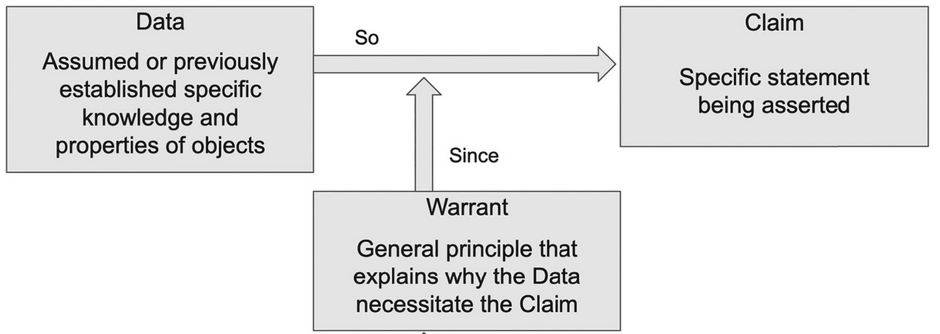
\includegraphics[width=0.5\textwidth]{../images/toulmin.png}
    \end{center}
    Helpful note: a warrant is a general principle and a data is a specific thing. For example, the group $G$ that we're thinking about is a data, and the statement ``group elements have inverses'' is a warrant.
\end{problem}


\subsection*{Subgroups of specific groups}

\begin{problem}
    Construct the subgroup lattice for $A_4$. Remember, this is the set of all the even permutations in $S_4$, so it consists of the following 12 elements:
    \begin{align*}
        0\text{-cycles: } &  () \\
        3\text{-cycles: } &  (1\; 2\; 3), (1\; 3\; 2), (1\; 2\; 4), (1\; 4\; 2),\\
        & (1\; 3\; 4), (1\; 4\; 3), (2\; 3\; 4), (2\; 4\; 3)\\
        \text{Double transpositions: } & (1\; 2)(3\; 4), (1\;3)(2\; 4), (1\; 4)(2\; 3)
    \end{align*}
    Notes:
    \begin{itemize}
        \item Why are 3-cycles even permutations? Note that for instance $(1\; 2\; 3) = (1\;2)(1\;3)$.
        \item Please use the permutation calculator or this will take forever. Make sure left-to-right multiplication is on.
        \item Start by finding all the cyclic subgroups. Then ``build up.''        
        \item I guarantee that all the subgroups will have order 1, 2, 3, 4, 6, or 12. (But I won't guarantee that there's subgroups of all those orders.)
    \end{itemize}
\end{problem}


\end{document}

